\documentclass[fontset=fandol]{ctexart}
\usepackage{graphicx}
\usepackage{float}
\usepackage{amsmath}
\usepackage{amsfonts} % 支持更多数学字体，并避免数学扩展字体的字号替换警告。
\usepackage{geometry}
\geometry{a4paper, centering,scale=0.8}
\usepackage[format=hang,font=small,textfont=it]{caption}
\usepackage[nottoc]{tocbibind}
\newcommand\degree{^\circ}
\title{\heiti 杂谈勾股定理}
\author{\kaishu Lysandra}
\date{\today} 
\bibliographystyle{plain}
\newenvironment{myquote}
    {\begin{quote}\kaishu\zihao{-5}}
    {\end{quote}}

\begin{document}

\maketitle
\begin{abstract}
这是一篇关于勾股定理的小短文
\end{abstract}
\tableofcontents
\section{勾股定理在古代}
西方称勾股定理为毕达哥拉斯定理，将勾股定理的发现归功于公元前 6 世纪的
毕达哥拉斯学派。\cite{Kline}该学派得到了一个法则，可以求出可排成直角三角形三边的三
元数组。毕达哥拉斯学派没有书面著作，该定理的严格表述和证明则见于欧几里
德\footnote{欧几里得，约公元前330--275年。}《几何原本》的命题 47：“直角三角形斜边上的正方形等于两直角边上的两
个正方形之和。”证明是用面积做的。

\begin{itemize}
    \item 几何
    \item 代数
\end{itemize}

\begin{description}
    \item[中文] 中国的语言文字
    \item[English] The language of the English-speaking world
    \item[Français] La langue française 
\end{description}
我国《周髀算经》载商高（约公元前 12 世纪）答周公问：
\begin{myquote}
勾广三，股修四，径隅五。
\end{myquote}
又载陈子（约公元前7--6世纪）答荣方问：
\begin{myquote} 
若求邪至日者，以日下为勾，日高为股，勾股各自乘，并而开方除之，得邪至日。
\end{myquote}
都较古希腊更早。

是我国古代对勾股定理的最早记载\cite{quanjing}。宋赵爽在《周髀算经注》中对勾股定理作了图解，给出了勾股定理的一个极具对称美的证明（见图\ref{fig:1}）。
\begin{figure}[ht]
    \centering
    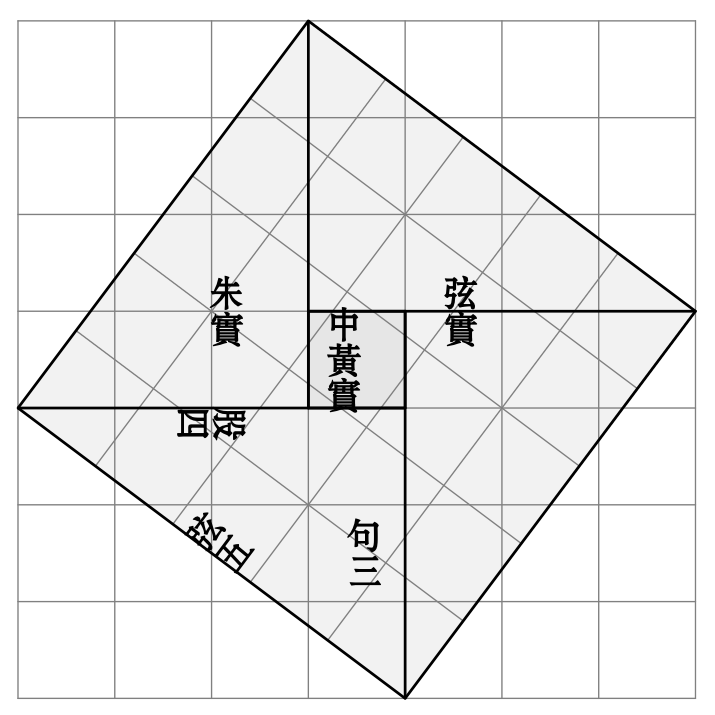
\includegraphics[scale=0.6]{1.png}
    \caption{宋赵爽在《周髀算经注》中对勾股定理的图解（仿制），该图给出了勾股定理的一个极具对称美的证明}
    \label{fig:1}
\end{figure}
\section{勾股定理}
\newtheorem{thm}{定理}
\begin{thm}[勾股定理]
直角三角形斜边的平方等于两直角边的平方和。

可以用符号语言表述为公式\ref{eq:gougu}
\begin{equation}\label{eq:gougu}
c^2 = a^2 + b^2
\end{equation}
满足式\ref{eq:gougu}的三元组 $(a, b, c)$ 称为\emph{勾股数}，下表列出一些较小的勾股数
\end{thm}
\begin{table}[H]
\begin{tabular}{|r|r|r|}
\hline
直角边 $a$ & 直角边 $b$ & 斜边 $c$ \\
\hline
    3 &     4 &     5 \\
    5 &    12 &    13 \\
    7 &    24 &    25 \\
\hline
\end{tabular}%
\qquad
($a^2 + b^2 = c^2$)
\end{table}
% 暂未在正文使用 \cite，先列出数据库中的全部文献。
\nocite{Shiye}
\bibliography{math}

\end{document}
